\documentclass[a4paper]{extarticle}
\usepackage[utf8]{inputenc}
\usepackage[a4paper, margin=1in]{geometry}

\usepackage{amssymb}
\usepackage{amsmath}
\usepackage{enumitem}
\usepackage{tcolorbox}
\usepackage{fancyhdr}
\usepackage{graphicx}
\usepackage{float}

\setlength{\parindent}{0em}
\setlength{\parskip}{0.4em}

\definecolor{theoremblue}{RGB}{1, 73, 124}
\definecolor{corollaryblue}{RGB}{70, 143, 175}
\definecolor{exampleblue}{RGB}{137, 194, 217}

\newtcolorbox{tbox}{colback=theoremblue!20,colframe=theoremblue,
boxrule=0pt,arc=0pt,boxsep=2pt,left=2pt,right=2pt,leftrule=2pt}

\newtcolorbox{cbox}{colback=corollaryblue!20,colframe=corollaryblue,
boxrule=0pt,arc=0pt,boxsep=2pt,left=2pt,right=2pt,leftrule=2pt}

\newtcolorbox{ebox}{colback=exampleblue!20,colframe=exampleblue,
boxrule=0pt,arc=0pt,boxsep=2pt,left=2pt,right=2pt,leftrule=2pt}

\title{IntroML - Lecture Notes Week 9}
\author{Ruben Schenk, ruben.schenk@inf.ethz.ch}
\date{\today}

\pagestyle{fancy}
\fancyhf{}
\rhead{ruben.schenk@inf.ethz.ch}
\rfoot{Page \thepage}
\lhead{IntroML - Lecture Notes Week 9}

\begin{document}

\maketitle

\section{Unsupervised Learning: Dimension Reduction}

\subsection{Introduction}

The basic challenge is posed as follows: Given a data set $D = \{x_1,..., \, x_n\}$ with $x_i \in \mathbb{R}^d$, obtain an \textbf{embedding} (low-dimensional representation) $z_1,..., \, z_n \in \mathbb{R}^k$ where typically $k << d$.

One might want to do this for several reasons:
\begin{itemize}
    \item Visualization ($k = 1, \, 2, \, 3$)
    \item Regularization (model selection)
    \item Unsupervised feature discovery (i.e. determining features from data)
    \item etc.
\end{itemize}

\textbf{Note:} Our focus is on model-based approaches, i.e.:
\begin{itemize}
    \item Given: Data $D = \{x_1,..., \, x_n\} \subseteq \mathbb{R}^d$
    \item Goal: Obtain a mapping $f : \mathbb{R}^d \to \mathbb{R}^k$ where usually $k << d$
    \item We can distinguish:
    \begin{itemize}
        \item Linear dimension reduction $f(x) = Ax$
        \item Nonlinear dimension reduction (parametric or non-parametric)
    \end{itemize}
\end{itemize}

\subsection{Dimension Reduction}

\textbf{Linear dimension redcution} can be seen as compression. The motivation behind this process is that low-dimensional representation should allow to compress the original data and allow for a accurate reconstruction.

Let us consider a simple example for $k = 1$. Given is a data set $D = \{x_1,..., \, x_n\} \subseteq \mathbb{R}^d$, assumed to be centered, i.e. $\mu = \frac{1}{n} \sum_i x_i = 0$. We want to represent the data as points on a line $x_i \approx z_iw$ with coefficients $w \in \mathbb{R}^d$.

\begin{figure}[H]
    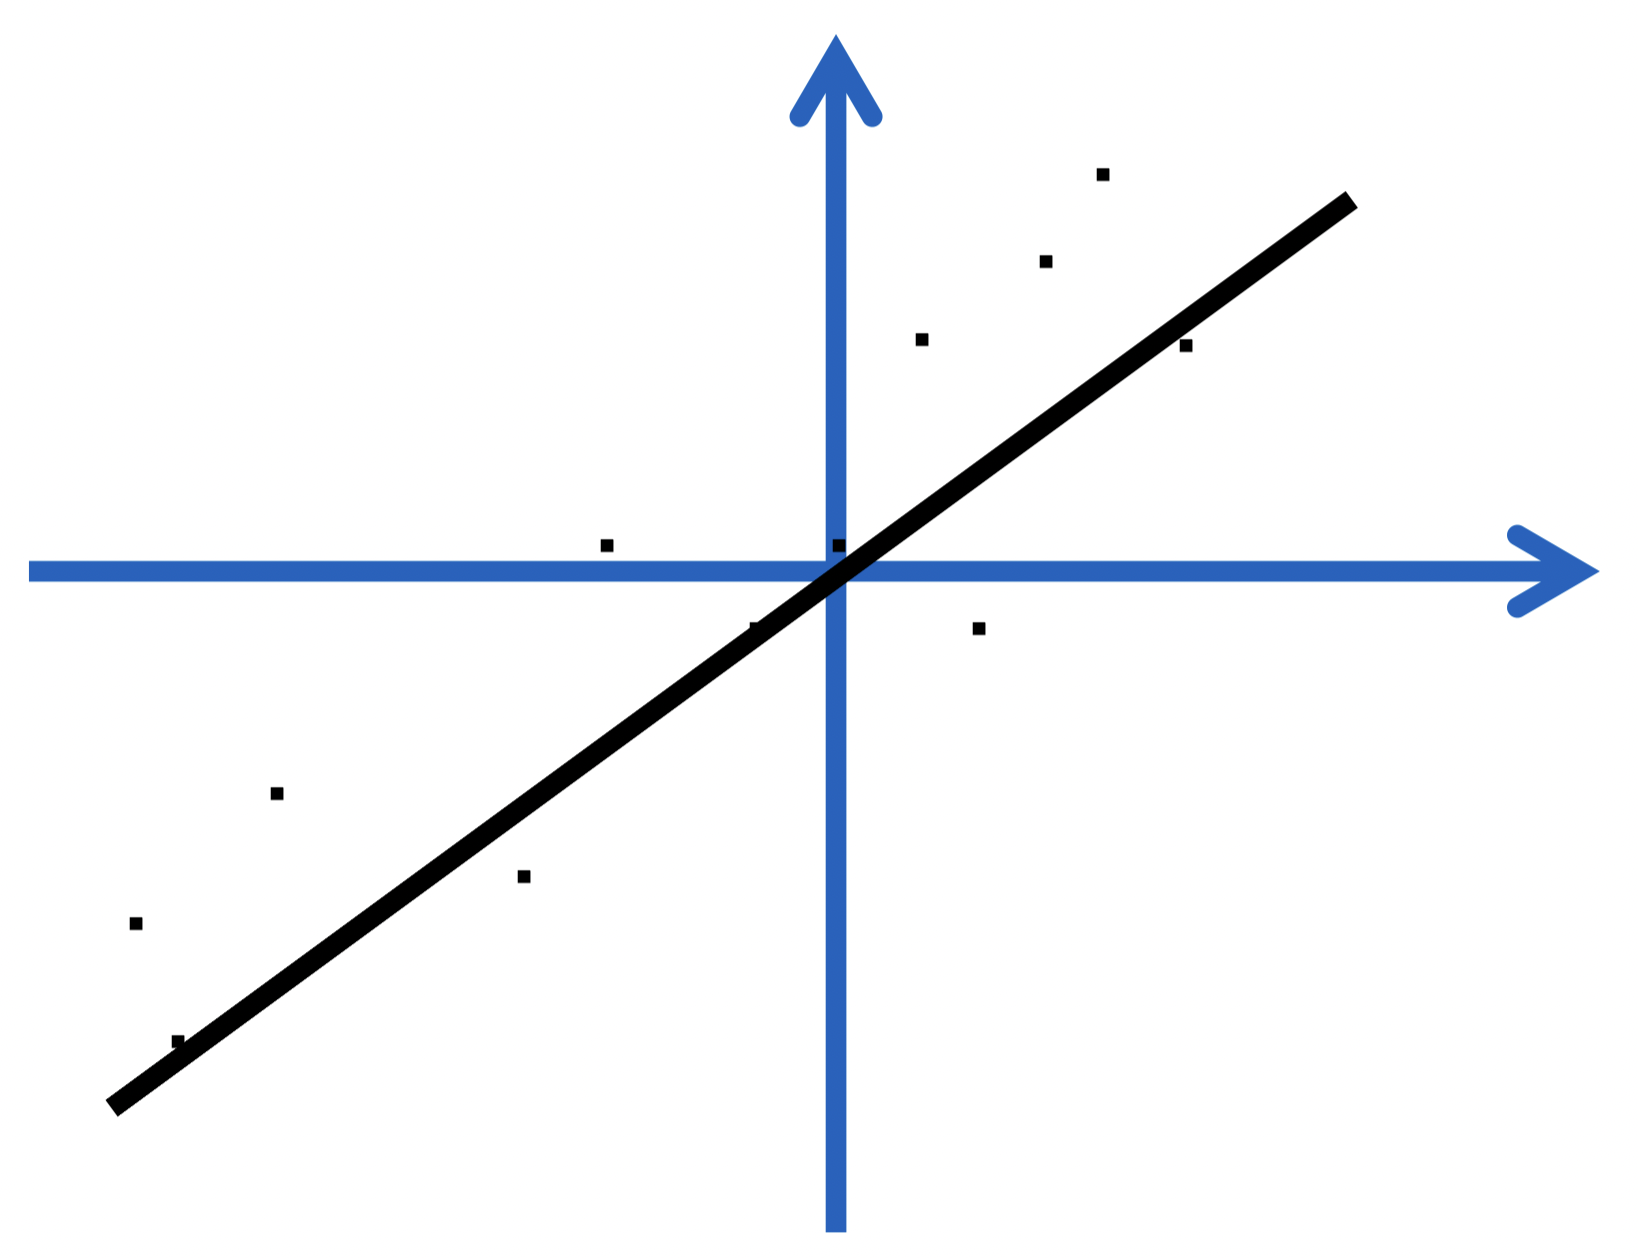
\includegraphics[width=5cm]{../images/IntroML_Fig9-1}
    \centering
\end{figure}

In other words, we want $x_i \approx z_iw$ minimizing $||z_iw - x_i||_2^2$. To ensure the uniqueness of the solution, we normalize $w$, i.e. $||w||_2 = 1$. We want to optimize jointly over $w, \, z_1, \, z_2,...$:

\[
    (w^*, \, z^*) = \arg \min_{||w||_2 = 1, \, z} \sum_{i = 1}^n ||z_iw - x_i||_2^2.
\]

In our $k = 1$ case, the optimal $z$ is given by:

\[
    z_i^* = w^Tx_i
\]

Thus, we effectively solve a \textit{regression} problem, interpreting $x$ as features and $z$ as labels. Since for any fixed $||w||_2 = 1$, it holds that $z_i^* = w^Tx_i$. Therefore, we only need:

\[
    w^* = \arg \min_{||w||_2 = 1} \sum_{i = 1}^n ||ww^Tx_i - x_i||_2^2,
\]
which is equivalent to
\[
    w^* = \arg \min_{||w||_2 = 1} \sum_{i = 1}^n (w^Tx_i)^2,
\]
which is furthermore equivalent to
\[
    w^* = \arg \max_{||w||_2 = 1} w^T\Sigma w,
\]
where $\Sigma = \frac{1}{n}\sum_{i = 1}^n x_ix_i^T$ is the \textit{empirical covariance,} assuming the data is centered (i.e. $\mu = \frac{1}{n} \sum_i x_i = 0$).

Finally, the optimal solution to $w^* = \arg \max_{||w||_2 = 1} w^T\Sigma w$ is given by the \textbf{principal eigenvector} of $\Sigma$, i.e. $w = v_1$ where, for $\lambda_1 \geq \cdots \geq \lambda_d \geq 0$,

\[
    \Sigma = \sum_{i = 1}^d \lambda_i v_i v_i^T.
\]

But what if $k > 1$? Suppose we wish to project more than one dimension. Thus we want:

\[
    (W, \, z_1,..., \, z_n) = \arg \min_{W^TW = I_k, \, z} \sum_{i = 1}^n ||Wz_i - x_i||_2^2,
\]

where $W \in \mathbb{R}^{d \times k}$ is \textit{orthogonal,} and $z_1,..., \, z_n \in \mathbb{R}^k$. This is called the \textit{principal component analysis} problem and its solution can be obtained in closed form even for $k > 1$.

\subsection{Principle Component Analysis (PCA)}

The \textbf{Principal Component Analysis (PCA)} problem is as follows:

Given centered data $D = \{x_1,..., \, x_n\} \subseteq \mathbb{R}^d$ with $\mu = \frac{1}{n} \sum_i x_i = 0$ and $\Sigma = \frac{1}{n} \sum_{i = 1}^n x_ix_i^T$, the solution to the PCA problem
\[
    (W, \, z_1,..., \, z_n) = \arg \min_{W^TW = I_k, \, z} \sum_{i = 1}^n ||Wz_i - x_i||_2^2,
\]
where $1 \leq k \leq d, \, W \in \mathbb{R}^{d \times k}$ is orthogonal and $z_1,..., \, z_n \in \mathbb{R}^k$, is given by

\[
    W = (v_1 \, | \, \cdots \, | \, v_k) \text{ and } z_i = W^Tx_i.
\]
Hereby: $\Sigma = \sum_{i = 1}^d \lambda_iv_iv_i^T$ and $\lambda_1 \geq \cdots \geq \lambda_d$.

The linear mapping $f(x) = W^Tx$ obtained from PCA \textit{projects} vectors $x \in \mathbb{R}^d$ into a $k$-dimensional subspace. This projection is chosen to \textit{minimize the reconstruction error} (measured in the Euclidean norm).

One might remember that we can obtain PCA through the \textit{Singular-Value Decomposition (SVD).} We recall that any $X \in \mathbb{R}^{n \times d}$ can be represented as

\[
    X = USV^T,
\]

where $U \in \mathbb{R}^{n \times n}$ and $V \in \mathbb{R}^{d \times d}$ are orthogonal, and $S \in \mathbb{R}^{n \times d}$ is diagonal (w.l.o.g. in decreasing order). Its entries are called \textit{singular values.} The top $k$ principal components are exactly the first $k$ columns of $V$:

\[
    n\Sigma = X^TX = VS^TU^TUSV^T = VS^TSV^T = VDV^T.
\]

Finally, we can compare PCA and k-means:

\textbf{PCA-Problem:}
\[
    (W, \, z_1,..., \, z_n) = \arg \min_{W^TW = I_k, \, z} \sum_{i = 1}^n ||Wz_i - x_i||_2^2,
\]
where $W \in \mathbb{R}^{d \times k}$ is \textit{orthogonal,} and $z_1,..., \, z_n \in \mathbb{R}^k$.

\textbf{k-means problem (equivalent formulation):}
\[
    (W, \, z_1,..., \, z_n) = \arg \min_{W, \, z} \sum_{i = 1}^n ||Wz_i - x_i||_2^2,
\]
where $W \in \mathbb{R}^{d \times k}$ is \textit{arbitrary,} and $z_1,..., \, z_n \in E_k$ for $E_k = \{e_1,..., \, e_k\}$ are all unit vectors.

In summary:
\begin{itemize}
    \item We can think of PCA and k-means as options to solve a similar unsupervised learning problem, with different constraints.
    \item Both aim to compress the data with maximum fidelity under constraints on the model complexity.
    \item This insight gives rise to a much broader class of techniques.
\end{itemize}

\subsection{Kernel PCA}

Recall that in supervised learning, kernels allowed us to solve non-linear problems by reducing them to linear ones in high-dimensional (implicitly represented) spaces. We can take the same approach for unsupervised learning!

Recall that the optimal solution to PCA problem solves for

\[
    w^* = \arg \max_{||w||_2 = 1} w^TX^TXw = \arg \max_{||w||_2} \sum_{i = 1}^n (w^Tx_i)^2.
\]

Applying feature maps, using $w = \sum_{j = 1}^n \alpha_j \phi(x_j)$ and observing that $||w||_2^2 = \alpha^TK\alpha$:

\begin{align*}
    \arg \max_{||w||_2 = 1} \sum_{i = 1}^n &= \arg \max_{\alpha^TK\alpha = 1} \sum_{i = 1}^n \Big(\sum_{j = 1}^n \alpha_j \phi(x_j)^T \phi(x_i) \Big)^2\\
    &= \arg \max_{\alpha^TK\alpha = 1} \sum_{i = 1}^n \Big(\sum_{j = 1}^n \alpha_j k(x_j, \, x_i) \Big)^2 \\
    &= \arg \max_{\alpha^TK\alpha = 1} \sum_{i = 1}^n (\alpha^TK_i)^2\\
    &= \arg \max_{\alpha^TK\alpha = 1} \alpha^TK^TK \alpha
\end{align*}

The \textbf{Kernel PCA} ($k = 1$) requires solving:

\[
    \alpha^* = \arg \max_{\alpha^Tk\alpha = 1} \alpha^TK^TK\alpha \equiv \arg \max_{\alpha} \frac{\alpha^TK^TK\alpha}{\alpha^TK\alpha}.
\]

The optimal solution is obtained in \textit{closed form} from the eigendecomposition of $K$:

\[
    \alpha^* = \frac{1}{\sqrt{\lambda_1}}v_1 \text{ for } K = \sum_{i = 1}^n \lambda_iv_iv_i^T \text{ and } \lambda_1 \geq \lambda_2 \geq \cdots \geq  \lambda_n \geq 0.
\]

For general $k \geq 1$, the \textbf{Kernel Principal Components} are given by $\alpha^{(1)},..., \, \alpha^{(k)} \in \mathbb{R}^n$, where

\[
    \alpha^{(i)} = \frac{1}{\sqrt{\lambda_i}}v_i
\]

is obtained from $K = \sum_{i = 1}^n \lambda_i v_i v_i^T$ and $\lambda_i \geq \lambda_2 \geq \cdots \geq \lambda_n$. Given this, a new point $x$ is projected as $z \in \mathbb{R}^k$, where

\[
    z_i = \sum_{j = 1}^n \alpha_j^{(i)}k(x_j, \, x).
\]

\textbf{Note:} Applying k-means or kernel-principal components is soemtimes called \textit{Kernel-k-means} or \textit{Spectral Clustering}.

Some notes on Kernel-PCA:
\begin{enumerate}
    \item Kernel-PCA corresponds to applying PCA in the feature space induced by the kernel $k$
    \item This can be used to discover non-linear feature maps in closed form
    \item This can be used as inputs, e.g. to SVMs given "multi-layer support vector machines"
    \item We may want to center the kernel, i.e. $K' = K - KE - EK + EKE$ where $E = \frac{1}{n}[1,..., \, 1][1,..., \, 1]^T$
\end{enumerate}

\subsection{Neural Network Autoencoders}

The problem with Kernel-PCA is that it requires data specified as a kernel:
\begin{itemize}
    \item Complexity grows with the number of data points
    \item Cannot easily "explicitly" embed high-dimensional data (unless we have an aapropriate kernel)
\end{itemize}

The key idea of \textbf{dimension reduction via Autoencoders} is to try and learn the idenity function $x \approx f(x; \, \theta)$. But what function $f$ should we pick?

\[
    f(x; \, \theta) = f_{dec}(f_{enc}(x; \, \theta_{enc}); \, \theta_{dec}),
\]

where $enc$ stands for "encoder" and $dec$ for "decoder". The idea is that the encoder maps the data to the lower-dimensional space and the decoder maps the data back to the original dimension:

\begin{figure}[H]
    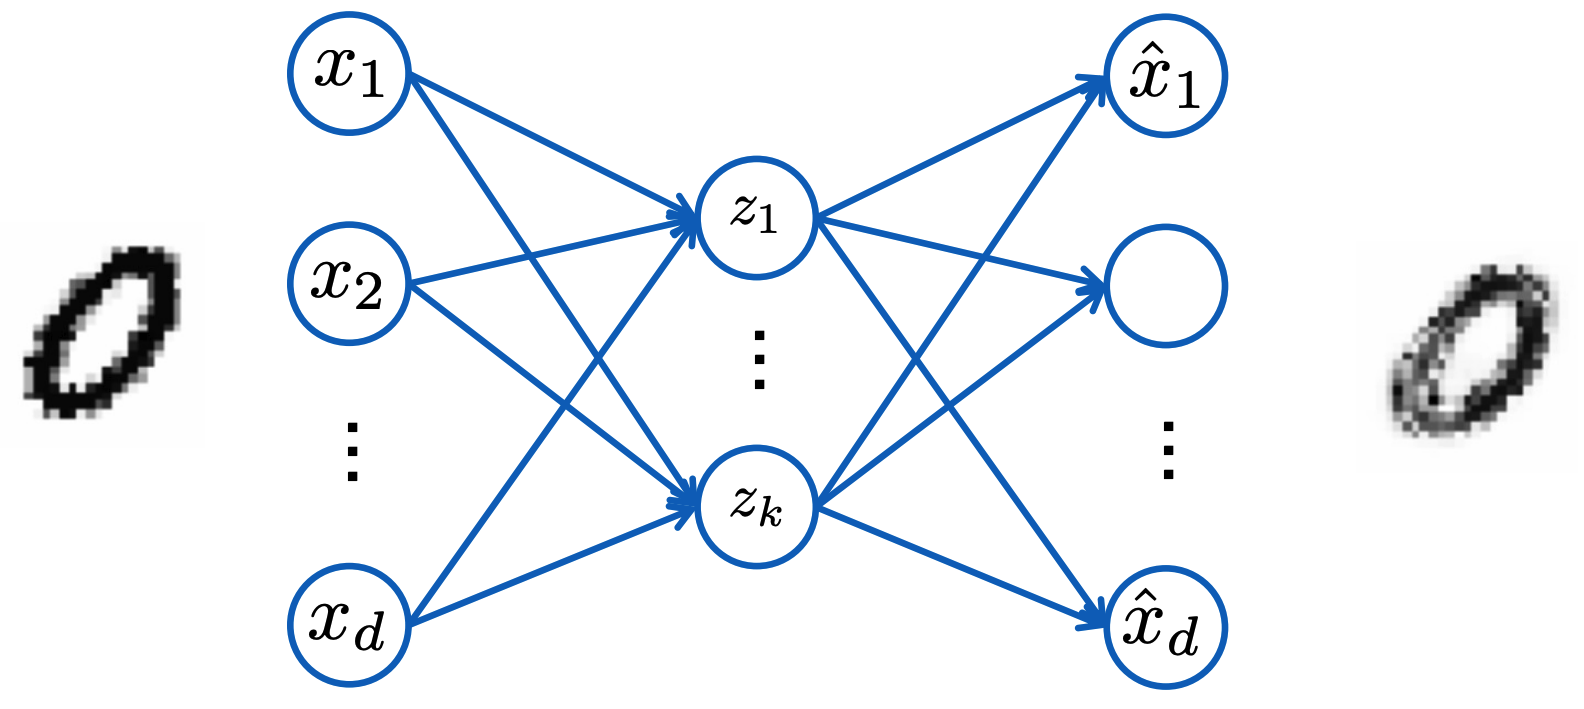
\includegraphics[width=15cm]{../images/IntroML_Fig9-2}
    \centering
\end{figure}

\textbf{Neural network Autoencoders} are ANNs where:
\begin{itemize}
    \item There is one output unit for each of the $d$ input units
    \item The number $k$ of hidden units is usually smaller than the number of inputs (the \textit{bottleneck})
\end{itemize}
The goal is to optimize the weights such that the \textit{output agrees with the input,} in other words minimizing the squared reconstruction error:

\[
    \min_W \sum_{i = 1}^n ||x_i - f(x_i; \, W)||_2^2.
\]

As seen in previous chapters, we can find a local minimum via SGD (backpropagation). If we compare Autoencoders to PCA, we see that the internal representation $z = \varPhi(W^{(enc)}x)$ is the "dimensionality reduced" input $x$. If the activation function is the identity, then in fact fitting a NN autoencoder is equivalent to PCA!

\subsection{Supervised vs. Unsupervised Learning}

\begin{figure}[H]
    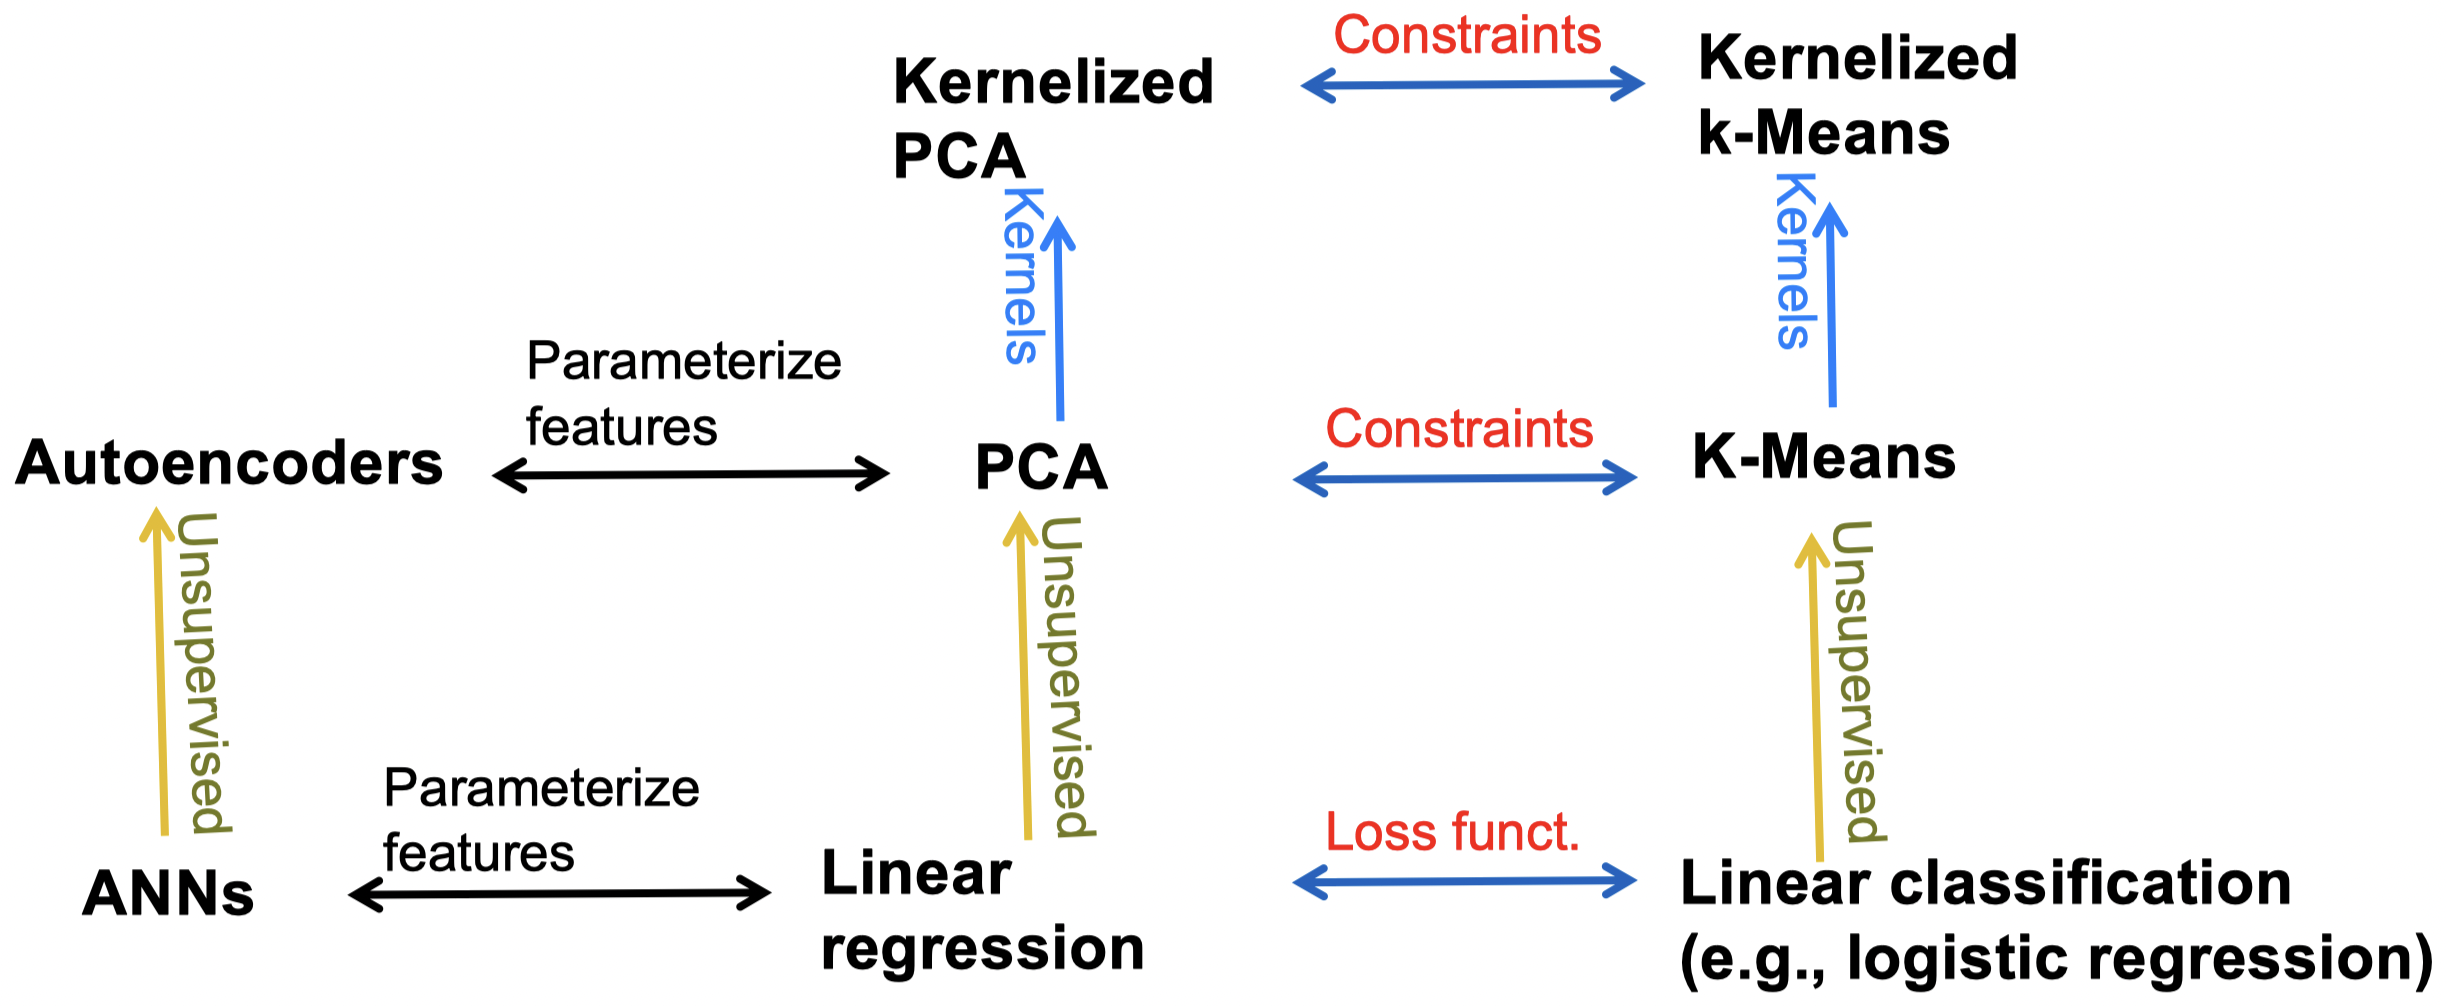
\includegraphics[width=15cm]{../images/IntroML_Fig9-3}
    \centering
\end{figure}

\begin{figure}[H]
    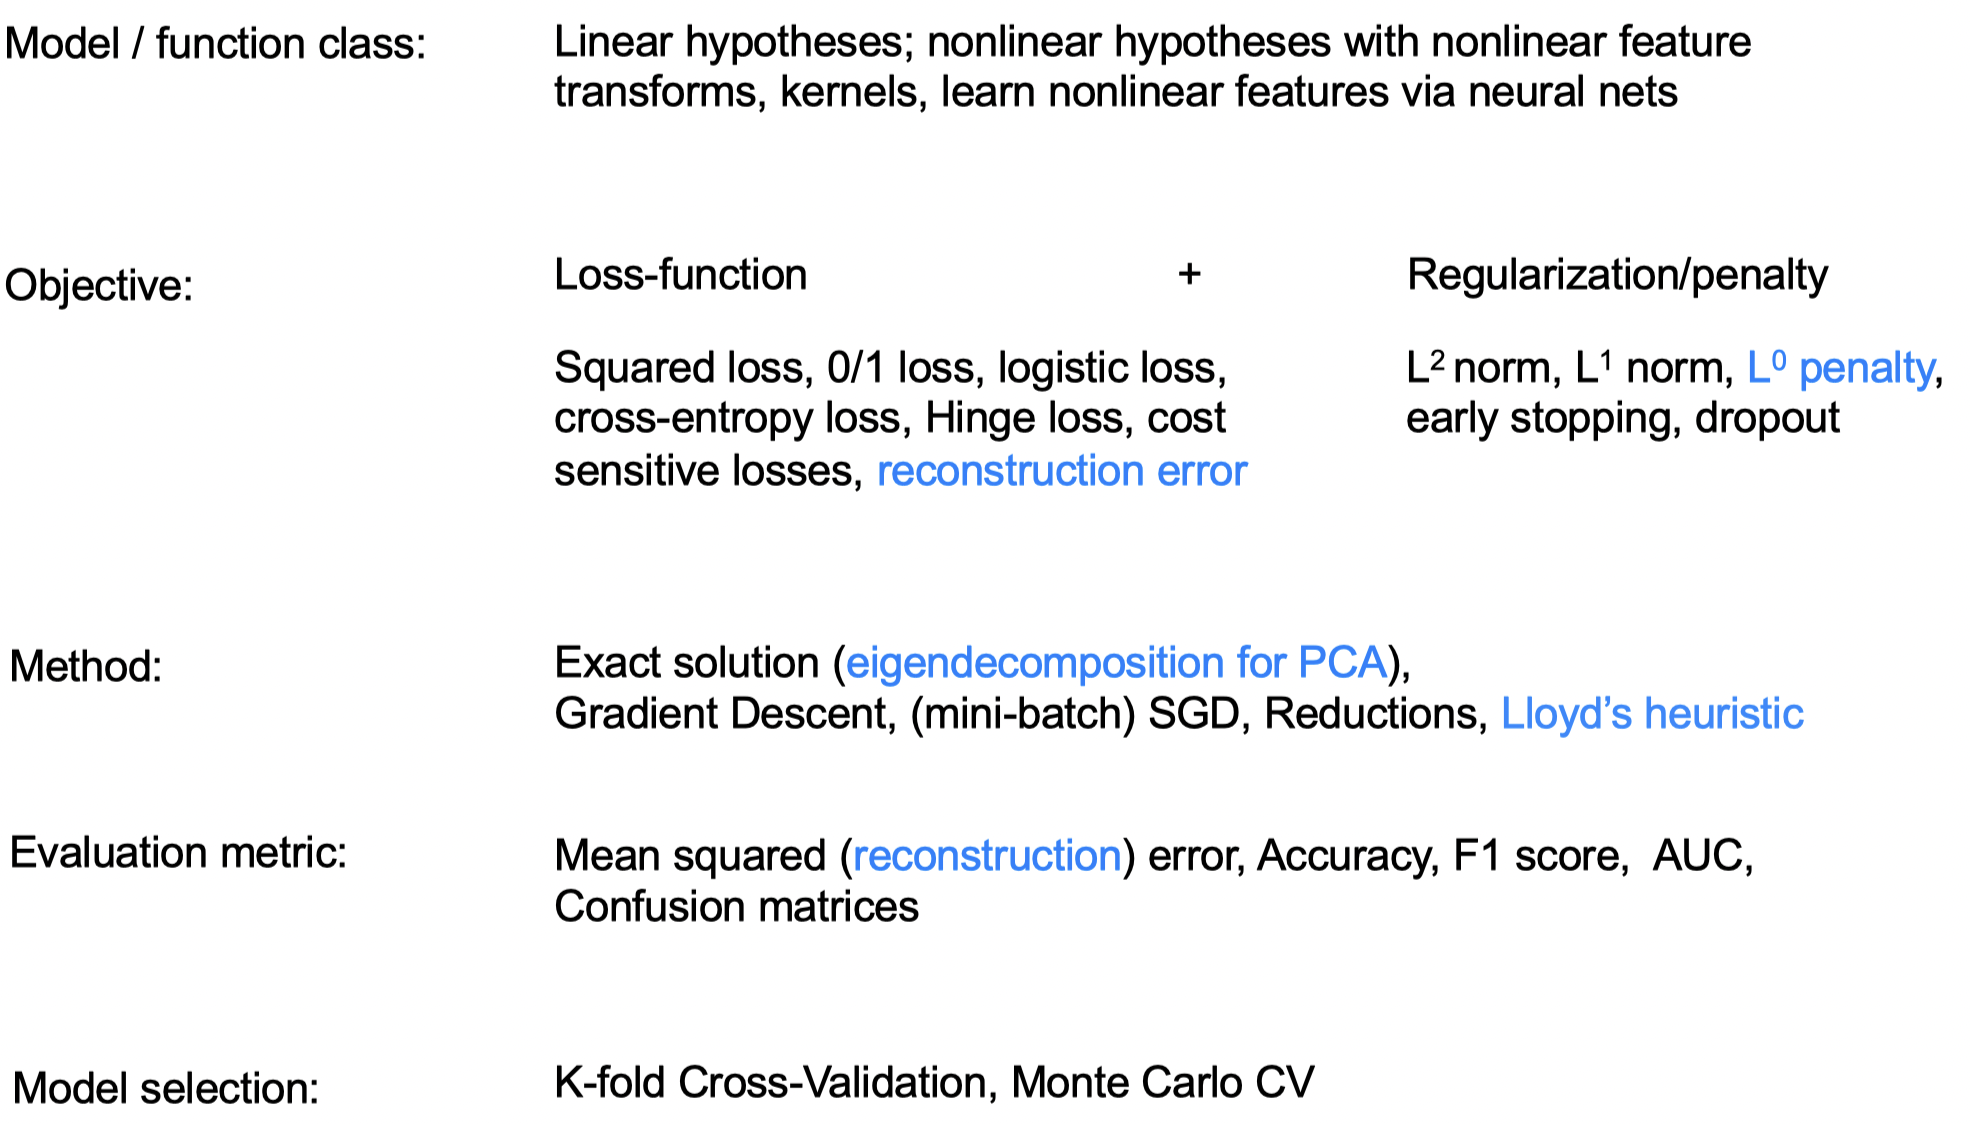
\includegraphics[width=15cm]{../images/IntroML_Fig9-4}
    \centering
\end{figure}

\end{document}